\documentclass{scrartcl} % scrartcl of scrreprt
% Include all project wide packages here.
\usepackage{fullpage}
\usepackage{polyglossia}
\setmainlanguage{dutch}
\usepackage{csquotes}
\usepackage{graphicx}
\usepackage{epstopdf}
\usepackage{pdfpages}
\usepackage{caption}
\usepackage[list=true]{subcaption}
\usepackage{float}
%\usepackage{mathtools}
\usepackage{standalone}
\usepackage{import}
\usepackage{tocloft}
\usepackage{wrapfig}
\usepackage{authblk}
\usepackage{array}
\usepackage{booktabs}
\usepackage[toc,page,title,titletoc]{appendix}
\usepackage{xunicode}
\usepackage{amsmath}
\usepackage{fontspec}
\usepackage{unicode-math}
\usepackage[
    backend=bibtexu,
	texencoding=utf8,
bibencoding=utf8,
    style=ieee,
    sortlocale=nl_NL,
    language=auto
]{biblatex}
\usepackage{listings}
\newcommand{\includecode}[3][c]{\lstinputlisting[caption=#2, escapechar=, style=#1]{#3}}
\newcommand{\superscript}[1]{\ensuremath{^{\textrm{#1}}}}
\newcommand{\subscript}[1]{\ensuremath{_{\textrm{#1}}}}


\newcommand{\chapternumber}{\thechapter}
\renewcommand{\appendixname}{Bijlage}
\renewcommand{\appendixtocname}{Bijlagen}
\renewcommand{\appendixpagename}{Bijlagen}

\usepackage[hidelinks]{hyperref} %<--------ALTIJD ALS LAATSTE

\renewcommand{\familydefault}{\sfdefault}

\setmainfont[Ligatures=TeX]{Myriad Pro}
\setmathfont{Asana Math}
\setmonofont{Lucida Console}

\usepackage{titlesec, blindtext, color}
\definecolor{gray75}{gray}{0.75}
\newcommand{\hsp}{\hspace{20pt}}
\titleformat{\chapter}[hang]{\Huge\bfseries}{\chapternumber\hsp\textcolor{gray75}{|}\hsp}{0pt}{\Huge\bfseries}
\renewcommand{\familydefault}{\sfdefault}
\renewcommand{\arraystretch}{1.2}
\setlength\parindent{0pt}

%For code listings
\definecolor{black}{rgb}{0,0,0}
\definecolor{browntags}{rgb}{0.65,0.1,0.1}
\definecolor{bluestrings}{rgb}{0,0,1}
\definecolor{graycomments}{rgb}{0.4,0.4,0.4}
\definecolor{redkeywords}{rgb}{1,0,0}
\definecolor{bluekeywords}{rgb}{0.13,0.13,0.8}
\definecolor{greencomments}{rgb}{0,0.5,0}
\definecolor{redstrings}{rgb}{0.9,0,0}
\definecolor{purpleidentifiers}{rgb}{0.01,0,0.01}


\lstdefinestyle{csharp}{
language=[Sharp]C,
showspaces=false,
showtabs=false,
breaklines=true,
showstringspaces=false,
breakatwhitespace=true,
escapeinside={(*@}{@*)},
columns=fullflexible,
commentstyle=\color{greencomments},
keywordstyle=\color{bluekeywords}\bfseries,
stringstyle=\color{redstrings},
identifierstyle=\color{purpleidentifiers},
basicstyle=\ttfamily\small}

\lstdefinestyle{c}{
language=C,
showspaces=false,
showtabs=false,
breaklines=true,
showstringspaces=false,
breakatwhitespace=true,
escapeinside={(*@}{@*)},
columns=fullflexible,
commentstyle=\color{greencomments},
keywordstyle=\color{bluekeywords}\bfseries,
stringstyle=\color{bluestrings},
identifierstyle=\color{purpleidentifiers}
}

\lstdefinestyle{vhdl}{
language=VHDL,
showspaces=false,
showtabs=false,
breaklines=true,
showstringspaces=false,
breakatwhitespace=true,
escapeinside={(*@}{@*)},
columns=fullflexible,
commentstyle=\color{greencomments},
keywordstyle=\color{bluekeywords}\bfseries,
stringstyle=\color{redstrings},
identifierstyle=\color{purpleidentifiers}
}

\lstdefinestyle{xaml}{
language=XML,
showspaces=false,
showtabs=false,
breaklines=true,
showstringspaces=false,
breakatwhitespace=true,
escapeinside={(*@}{@*)},
columns=fullflexible,
commentstyle=\color{greencomments},
keywordstyle=\color{redkeywords},
stringstyle=\color{bluestrings},
tagstyle=\color{browntags},
morestring=[b]",
  morecomment=[s]{<?}{?>},
  morekeywords={xmlns,version,typex:AsyncRecords,x:Arguments,x:Boolean,x:Byte,x:Char,x:Class,x:ClassAttributes,x:ClassModifier,x:Code,x:ConnectionId,x:Decimal,x:Double,x:FactoryMethod,x:FieldModifier,x:Int16,x:Int32,x:Int64,x:Key,x:Members,x:Name,x:Object,x:Property,x:Shared,x:Single,x:String,x:Subclass,x:SynchronousMode,x:TimeSpan,x:TypeArguments,x:Uid,x:Uri,x:XData,Grid.Column,Grid.ColumnSpan,Click,ClipToBounds,Content,DropDownOpened,FontSize,Foreground,Header,Height,HorizontalAlignment,HorizontalContentAlignment,IsCancel,IsDefault,IsEnabled,IsSelected,Margin,MinHeight,MinWidth,Padding,SnapsToDevicePixels,Target,TextWrapping,Title,VerticalAlignment,VerticalContentAlignment,Width,WindowStartupLocation,Binding,Mode,OneWay,xmlns:x}
}

%defaults
\lstset{
basicstyle=\ttfamily\small,
extendedchars=false,
numbers=left,
numberstyle=\ttfamily\tiny,
stepnumber=1,
tabsize=4,
numbersep=5pt
}
\addbibresource{../../library/bibliography.bib}

\author{}
\title{EPO3: Eindrapport - Ontwerp}

\begin{document}
\chapter{Systeemoverzicht}
\label{ch:ontwerp}

Het uiteindelijke ontwerp is te zien in figuur~\ref{fig:ontwerp-schema}. In het schema staat hoe de GPU is verdeeld en staat wat voor onderlinge interacties er plaatsvinden tussen de modules.
Elke module is een component van de GPU met zijn eigen in VHDL beschreven gedrag en met zijn eigen functie. De screenbuffers zitten in het externe VRAM. 
\\
De GPU is verdeeld in 5 modules: de SPI, de Instructiedecoder, de Draw-logic, de RAM-controller en de VGA-controller. Daarbij is de Draw-logic module nog verdeeld in modules om de verschillende functies voor verschillende vormen te representeren. Er zijn vier modules: draw\_pixel, draw\_rect, draw\_line en draw\_sprite. Deze modules tekenen respectievelijk een pixel, rechthoek (contour of gevuld), lijn of sprite in de screenbuffer.
\\
Wat er precies gebeurt in de modules zal uitgelegd worden bij de hoofdstukken met de naam van de desbetreffende module. In dit hoofdstuk zal de nadruk liggen op de interacties tussen de modules.

\section{CPU --> SPI}
De SPI (slave) ontvangt via zijn verbinding met de SPI-module op de CPU (master) de benodigde data om iets te tekenen binnen, oftewel een instructie. Deze SPI-verbinding bestaat uit een CLK en een MOSI (master out, slave in) signaal, er is hier geen MISO (master in, slave out) signaal gebruikt, omdat er geen data teruggestuurd hoeft te worden naar de CPU. Het CLK signaal is de klok waarop het verzenden van data tussen de SPI modules is gesynchroniseerd. Een klokslag betekent dat er een nieuwe bit op de MOSI ingang is gezet, klaar om gelezen te worden. 
SPI implementeert normaal gesproken ook een SS (slave select) ingang, maar aangezien wij met slechts één slave werken, hebben we op deze ingang bespaard.

\section{SPI <--> Instructiedecoder}
De SPI verstuurt de ontvangen data naar de instructiedecoder in 8-bit pakketjes, samen met een signaal dat aangeeft dat er nieuwe data beschikbaar is. De SPI krijgt dan een reset-signaal van de instructiedecoder, wanneer het pakketje volledig binnen is gekomen, om de stabiliteit te verhogen.

\section{Instructiedecoder --> CPU}
De instructiedecoder stuurt direct een signaal naar de CPU om aan te geven wanneer de GPU klaar is voor een volgende instructie.

\section{Instructiedecoder <--> Draw-logic}
Nadat de instructiedecoder alle instructiedata van de CPU ontvangen heeft, stuurt hij de data naar de Draw-logic en schakelt hij de correcte module in. Draw-logic geeft zijn status weer aan de instructiedecoder middels een draw\_ready signaal dat aangeeft of Draw-logic zijn volgende instructie kan verwerken of nog steeds bezig is met een instructie.

\section {Instructiedecoder <--> RAM-controller en VRAM}
Voor het inladen van sprites in het VRAM, geeft de instructiedecoder aan bij de RAM-controller dat hij wil schrijven, om te voorkomen dat andere modules tegelijkertijd dingen in of uit het VRAM gaan lezen of schrijven. De RAM-controller stuurt het signaal decoder\_can\_access naar de instructiedecoder dat verteld of RAM-controller bezig is met instructies van een andere module.

\section {Instructiedecoder --> Draw-logic \& VGA-controller}
De instructiedecoder stuurt het ASB signaal naar de Draw-logic en de VGA-controller om ervoor te zorgen dat de juiste instructie in het juiste screenbuffer wordt gelezen of geschreven. De instructiedecoder bepaald hiermee in welk screenbuffer wordt geschreven en uit welke screenbuffer wordt gelezen.

\section {Draw-logic <--> Modules}
Draw-logic verstuurt de verkregen instructies van de instructiedecoder naar de juiste module. De desbetreffende module stuurt dan, de naar pixels verwerkte instructie, terug naar de Draw-logic met een signaal dat het klaar is met het verwerken van de instructie en dus klaar is voor de volgende instructie.

\section {Draw-logic <--> RAM-controller en VRAM}
Draw-logic geeft bij de RAM-controller aan dat hij wil lezen of schrijven, zodat andere modules dat niet tegelijkertijd ook kunnen doen. Vervolgens kan de gactiveerde draw-module zijn pixeldata naar het VRAM schrijven, in het juiste screen buffer.

\section{RAM-controller <--> VRAM}
Wanneer er geschreven kan worden naar het VRAM zet de RAM-controller het signaal write-enable op hoog, zodat de data die op dat moment op de ramdata-bus staat wordt geschreven naar het adres wat op dat moment in de ramaddr-bus staat.

\section{VGA-controller <--> RAM-controller}
Wanneer het volgende frame op het beeldscherm getekend moet worden, geeft de VGA-controller bij de RAM-controller aan dat hij wil lezen. Vervolgens wordt het gehele actieve schermbuffer uitgelezen en op de ramdata-bus gezet.

\section{VGA-controller --> Externe VGA-DAC}
De VGA-controller stuurt vgahsync, vgavsync en vga\_claim naar de Externe VGA DAC. De vgahsync en vgavsync zijn signalen die zorgen voor de juiste VGA timing die nodig is om de monitor juist aan te sturen voor een vloeiend beeld. De vga\_claim komt als het signaal vga\_enabled aan bij de VGA-DAC, zodat het weet dat de er een screenbuffer uitgelezen gaat worden. De VGA-DAC zet de data uit de ramdata-bus op het beeldscherm.

\section{Parameters} 
In bijlage~\ref{app:parameters} staat een overzicht van de gebruikte parameters en generics uit onze GPU.

%Aanpassen deze figuur
\begin{figure}[H]
\centering
	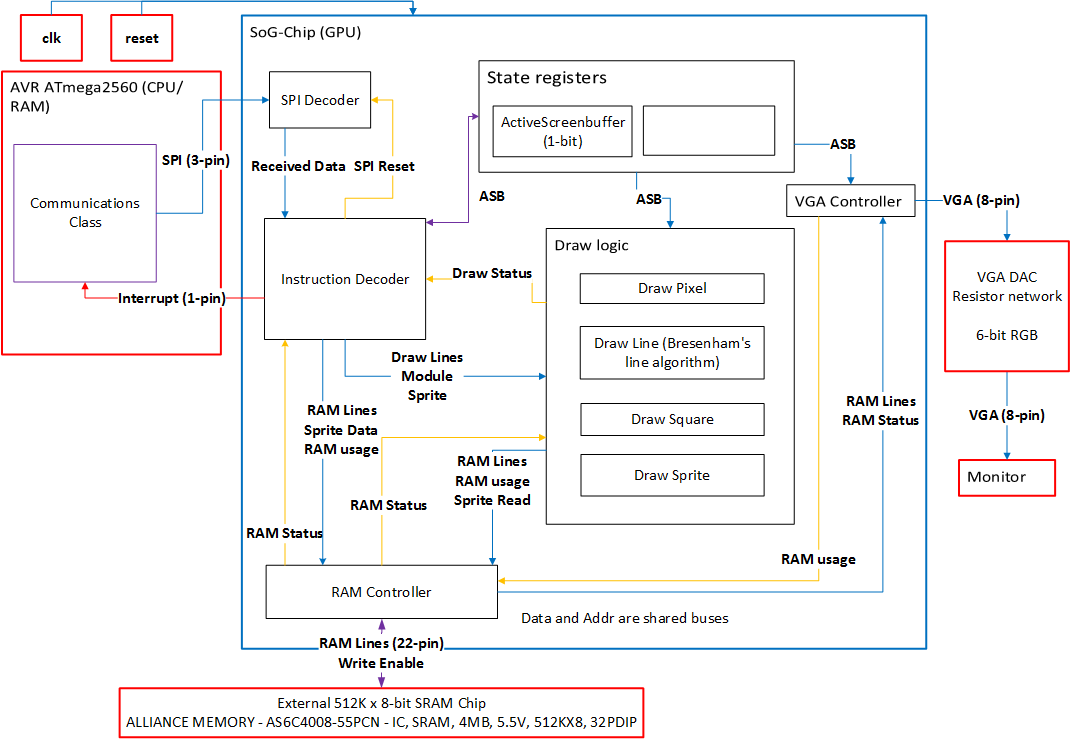
\includegraphics[scale=0.9, angle=90]{resource/systeemdrawing-detail.png}
	\caption{Ontwerp GPU}
	\label{fig:ontwerp-schema}
\end{figure}


% \section{SPI Controller}
% Voor de communicatie tussen de AVR en onze GPU hebben we een SPI decoder nodig.
% De ingang SS staat voor slave select, deze wordt normaal gebruikt voor het geval dat je meerdere slave chips hebt, aangezien dit bij ons niet het geval is zal dit signaal altijd hoog zijn.
% De in- en uitgangen zijn gespecificeerd in Tabel \ref{tab:spec-spi}.

% \begin{table}[H]
% \centering
% \caption{Specificaties van de SPI Controller (spi)}
% \label{tab:spec-spi}
% \begin{tabular}{c c c}
% 	\hline\hline
%  	Naam & Modus & Type\\
%  	\hline
% 	clk & in & std\_logic \\
% 	reset & in & std\_logic \\
% 	spi\_clk & in & std\_logic \\
% 	spi\_ss & in & std\_logic \\
% 	spi\_mosi & in & std\_logic \\
% 	spi\_data\_available & out & std\_logic \\
% 	spi\_data\_rx & out & std\_logic\_vector(SizeSPIData-1 downto 0) \\
%   	\hline
% \end{tabular}
% \end{table}

% \section{Instruction Decoder}
% De instructiedecoder is er om de door de AVR geleverde data te vertalen naar data (een instructie), waar de draw-module mee over weg kan.
% De decoder leest van SPI-interface een byte (SPIDataRxd), wanneer de SPI-interface aangeeft dat deze klaar staat (SPIDataAvailable).
% Deze byte wordt vervolgens afhankelijk van een interne counter vertaald naar een instructie, kleur of coördinaat.
% Wanneer de decoder met zijn ingebouwde counter bepaalt dat de instructiedata (één of meer bytes) geheel ontvangen is, wordt de bijbehorende actie ondernomen.
% Dit houdt in dat de gewenste draw-module wordt geactiveerd (met het signaal en), of het screen buffer wordt omgewisseld (reg\_id, reg\_value, reg\_set).
% Het actieve screen buffer wordt bijgehouden in een globaal register.
% Dit alles gebeurt uiteraard geheel synchroon en uitgangsdata blijft beschikbaar tot de volgende instructie door middel van flip-flops.
% De in- en uitgangen zijn gespecificeerd in Tabel \ref{tab:spec-decoder}.

% \begin{table}[H]
% \centering
% \caption{Specificaties van de Insctructie Decoder (decoder)}
% \label{tab:spec-decoder}
% \begin{tabular}{c c c}
% 	\hline\hline
%  	Naam & Modus & Type\\
%  	\hline
% 	clk & in & std\_logic \\
% 	reset & in & std\_logic \\	
% 	spi\_data\_rx & out & std\_logic\_vector(SizeSPIData-1 downto 0) \\
% 	spi\_data\_available & in & std\_logic \\
% 	draw\_ready & in & std_logic\\ 	
% 	x &  buffer & std\_logic\_vector(SizeX-1 downto 0) \\
% 	w &  buffer & std\_logic\_vector(SizeX-1 downto 0) \\
% 	y &  buffer & std\_logic\_vector(SizeY-1 downto 0) \\
% 	h &  buffer & std\_logic\_vector(SizeY-1 downto 0) \\
% 	color &  buffer & std\_logic\_vector(SizeColor-1 downto 0) \\
% 	id &  buffer & std\_logic\_vector(SizeSpriteID-1 downto 0) \\
% 	en & buffer & std\_logic\_vector(NumDrawModules-1 downto 0)\\
% 	asb & buffer & std\_logic \\ 
% 	int\_ready & out & std\_logic \\
% 	decoder\_can\_access & in & std\_logic \\
% 	decoder\_claim & out & std\_logic \\
% 	is\_init & out & std\_logic \\
% 	 ramaddr & out & std\_logic\_vector(SizeRAMAddr-1 downto 0) \\
% 	 ramdata & out & std\_logic\_vector(SizeRAMData-1 downto 0) \\
%   	\hline
% \end{tabular}
% \end{table}

% \section{Draw Module}
% In dit module worden de instructie omgezet naar pixels, rechthoeken en lijnen, die met kleur gevuld kunnen worden.
% Dit module krijgt de informatie binnen van de instructiedecoder, deze geeft aan welke module er gebruikt moet worden met de bijbehorende data (x, y, etc.), ook is er een input die het huidige screen buffer aanduidt (asb).
% De draw module schijft naar het niet-actieve screenbuffer.
% Verder bevat de module de benodigde signals om naar het RAM te schrijven (ramaddr en ramdata) en om te bepalen of er naar het RAM geschreven kan worden op een bepaald moment (draw\_write, draw\_read, draw\_can\_access).

% De in- en uitgangen zijn gespecificeerd in Tabel \ref{tab:spec-draw}.

% \begin{table}[H]
% \centering
% \caption{Specificaties van de Draw Module (draw)}
% \label{tab:spec-draw}
% \begin{tabular}{c c c}
% 	\hline\hline
%  	Naam & Modus & Type\\
%  	\hline	
% 	 clk & in & std\_logic \\
% 	 reset & in & std\_logic \\
% 	id & in & std\_logic\_vector(SizeSpriteID-1 downto 0) \\
% 	 x & in & std\_logic\_vector(SizeX-1 downto 0) \\ 
% 	 w & in & std\_logic\_vector(SizeX-1 downto 0) \\
% 	 y & in & std\_logic\_vector(SizeY-1 downto 0) \\
% 	 h & in & std\_logic\_vector(SizeY-1 downto 0) \\ 
% 	 color & in & std\_logic\_vector(SizeColor-1 downto 0) \\ 
% 	 en & in & std\_logic\_vector(NumDrawModules-1 downto 0) \\ 
% 	 draw\_ready & out & std\_logic \\
% 	 asb & in & std\_logic \\ 
% 	 draw\_write & out & std\_logic \\
% 	 draw\_read & out & std\_logic \\
% 	 draw\_can\_access & in & std\_logic \\
% 	 ramaddr & out & std\_logic\_vector(SizeRAMAddr-1 downto 0) \\
% 	 ramdata & out & std\_logic\_vector(SizeRAMData-1 downto 0) \\
%   	\hline
% \end{tabular}
% \end{table}

% \subsection {Fill}
% De Fill-module verandert in één instructie het hele beeldscherm naar een gegeven kleur.

% \begin{table}[H]
% \centering
% \caption{Specificaties van de Fill Draw Module}
% \label{tab:spec-fill-draw}
% \begin{tabular}{c c c}
% 	\hline\hline
%  	Naam & Modus & Type\\
%  	\hline	
% 	clk & in & std\_logic \\
% 	reset & in & std\_logic \\
% 	enable& in & std\_logic \\
% 	color & in & std\_logic\_vector(SizeColor-1 downto 0) \\
% 	asb & in & std\_logic \\
% 	done & out & std\_logic \\
% 	ramaddr &out & std\_logic\_vector(SizeRAMAddr-1 downto 0) \\
% 	ramdata &out & std\_logic\_vector(SizeRAMData-1 downto 0) \\
% 	draw\_write &out & std\_logic \\
% 	draw\_can\_access & in & std\_logic \\
%   	\hline
% \end{tabular}
% \end{table}

% \subsection {Pixel}
% Door deze module worden aparte pixels getekend, hiervoor zijn de x- en y-coördinaten en de kleur van de pixel nodig.

% \begin{table}[H]
% \centering
% \caption{Specificaties van de Pixel Draw Module}
% \label{tab:spec-pixel-draw}
% \begin{tabular}{c c c}
% 	\hline\hline
%  	Naam & Modus & Type\\
%  	\hline	
% 	clk & in & std\_logic \\
% 	reset & in & std\_logic \\
% 	enable& in & std\_logic \\
% 	color & in & std\_logic\_vector(SizeColor-1 downto 0) \\
% 	x & in & std\_logic\_vector(SizeX-1 downto 0) \\
% 	y & in & std\_logic\_vector(SizeY-1 downto 0) \\
% 	asb & in & std\_logic \\
% 	done & out & std\_logic \\
% 	ramaddr &out & std\_logic\_vector(SizeRAMAddr-1 downto 0) \\
% 	ramdata &out & std\_logic\_vector(SizeRAMData-1 downto 0) \\
% 	draw\_write &out & std\_logic \\
% 	draw\_can\_access & in & std\_logic \\
%   	\hline
% \end{tabular}
% \end{table}

% \subsection {Line}
% Deze module kan lijnen tekenen aan de hand van 2 coördinaten. Met deze coördinaten wordt er gerekend aan de hand van Bresenham's lijn algoritme welke pixels nodig zijn om de 2 coördinaten met een lijn te verbinden.

% \begin{table}[H]
% \centering
% \caption{Specificaties van de Line Draw Module}
% \label{tab:spec-line-draw}
% \begin{tabular}{c c c}
% 	\hline\hline
%  	Naam & Modus & Type\\
%  	\hline	
% 	clk & in & std\_logic \\
% 	reset & in & std\_logic \\
% 	enable& in & std\_logic \\
% 	color & in & std\_logic\_vector(SizeColor-1 downto 0) \\
% 	x0 & in & std\_logic\_vector(SizeX-1 downto 0) \\
% 	y0 & in & std\_logic\_vector(SizeY-1 downto 0) \\
% 	x1 & in & std\_logic\_vector(SizeX-1 downto 0) \\
% 	y1 & in & std\_logic\_vector(SizeY-1 downto 0) \\
% 	asb & in & std\_logic \\
% 	done & out & std\_logic \\
% 	ramaddr &out & std\_logic\_vector(SizeRAMAddr-1 downto 0) \\
% 	ramdata &out & std\_logic\_vector(SizeRAMData-1 downto 0) \\
% 	draw\_write &out & std\_logic \\
% 	draw\_can\_access & in & std\_logic \\
%   	\hline
% \end{tabular}
% \end{table}

% \subsection {Rectangle}
% In deze module wordt een rechthoek getekend met de x- en y-coördinaten van de eerste pixel links boven en de gegeven afmetingen. De rechthoek kan ook met kleur ingevuld worden. 

% \begin{table}[H]
% \centering
% \caption{Specificaties van de Rectangle Draw Module}
% \label{tab:spec-rect-draw}
% \begin{tabular}{c c c}
% 	\hline\hline
%  	Naam & Modus & Type\\
%  	\hline	
% 	clk & in & std\_logic \\
% 	reset & in & std\_logic \\
% 	enable& in & std\_logic \\
% 	enablef& in & std\_logic \\
% 	color & in & std\_logic\_vector(SizeColor-1 downto 0) \\
% 	x & in & std\_logic\_vector(SizeX-1 downto 0) \\
% 	y & in & std\_logic\_vector(SizeY-1 downto 0) \\
% 	w & in & std\_logic\_vector(SizeX-1 downto 0) \\
% 	h & in & std\_logic\_vector(SizeY-1 downto 0) \\
% 	asb & in & std\_logic \\
% 	done & out & std\_logic \\
% 	ramaddr &out & std\_logic\_vector(SizeRAMAddr-1 downto 0) \\
% 	ramdata &out & std\_logic\_vector(SizeRAMData-1 downto 0) \\
% 	draw\_write &out & std\_logic \\
% 	draw\_can\_access & in & std\_logic \\
%   	\hline
% \end{tabular}
% \end{table}

% \subsection {Sprite}
% In deze module wordt een sprite uitgelezen/ingeschreven vanuit het RAM en getekend op het scherm aan de hand van de x- en y- coördinaten van de eerste pixel links boven en de lengte, deze lengte geeft aan hoeveel adressen lang de sprite is.
% \begin{table}[H]
% \centering
% \caption{Specificaties van de Sprite Draw Module}
% \label{tab:spec-sprite-draw}
% \begin{tabular}{c c c}
% 	\hline\hline
%  	Naam & Modus & Type\\
%  	\hline	
% 	clk & in & std\_logic \\
% 	reset & in & std\_logic \\
% 	enable& in & std\_logic \\
% 	id & in & std\_logic\_vector(SizeSpriteID-1 downto 0) \\
% 	color & in & std\_logic\_vector(SizeColor-1 downto 0) \\
% 	x & in & std\_logic\_vector(SizeX-1 downto 0) \\
% 	y & in & std\_logic\_vector(SizeY-1 downto 0) \\
% 	w & in & std\_logic\_vector(SizeX-1 downto 0) \\
% 	l & in & std\_logic\_vector(SizeSpriteCounter-1 downto 0) \\
% 	asb & in & std\_logic \\
% 	done & out & std\_logic \\
% 	ramaddr &out & std\_logic\_vector(SizeRAMAddr-1 downto 0) \\
% 	ramdata &out & std\_logic\_vector(SizeRAMData-1 downto 0) \\
% 	draw\_write &out & std\_logic \\
% 	draw\_read &out & std\_logic \\
% 	draw\_can\_access & in & std\_logic \\
%   	\hline
% \end{tabular}
% \end{table}

% \section{RAM-controller}
% Omdat we een externe RAM gebruiken voor onze screenbuffers is het nodig om hiervoor communicatie op te stellen, zodat er in het juiste gedeelte van de RAM geschreven en gelezen wordt en dat dit niet tegelijkertijd gebeurd, omdat het RAM dat niet aankan. We hebben voor een externe RAM gekozen omdat er geen RAM geheugen groot genoeg gemaakt kon worden met de benodigde transistoren om bijvoorbeeld de screenbuffers te renderen. De RAM-controller stuurt naar het draw-module een signaal write als het mag gaan schrijven in het RAM geheugen, de RAM-controller krijgt dan de kleur en het adress binnen van het draw-module. Als de VGA-controller mag gaan lezen krijgt het een signaal read binnen van de RAM-controller dan zal er weer data naar de VGA-controller verstuurd worden, kleur en adres.

% \begin{table}[H]
% \centering
% \caption{Specificaties van de RAM-controller (ramcontroller)}
% \label{tab:spec-ramcontroller}
% \begin{tabular}{c c c}
% 	\hline\hline
%  	Naam & Modus & Type\\
%  	\hline	
% 	write\_enable & out & std\_logic\\
% 	vga\_claim & in & std\_logic\\
% 	decoder\_claim & in & std\_logic\\
% 	is\_init & in & std\_logic\\
% 	decoder\_write & in & std\_logic\\
% 	draw\_write & in & std\_logic\\
% 	draw\_read & in & std\_logic\\
% 	vga\_read & in & std\_logic\\
% 	draw\_can\_access & out & std\_logic\\
% 	decoder\_can\_access & out & std\_logic\\
% 	vga\_can\_access & out & std\_logic\\
%   	\hline
% \end{tabular}
% \end{table}

% \section{VGA-controller}
% De VGA-controller leest het actieve screen buffer uit het RAM en zet de gelezen data om in beelduitvoer.

% \begin{table}[H]
% \centering
% \caption{Specificaties van de VGA-controller (vgacontroller)}
% \label{tab:spec-vgacontroller}
% \begin{tabular}{c c c}
% 	\hline\hline
%  	Naam & Modus & Type\\
%  	\hline	
% 	clk & in & std\_logic \\ 
% 	reset\_n & in & std\_logic \\ 
% 	vgahsync & out & std\_logic \\ 
% 	vgavsync & out & std\_logic \\ 
% 	vgacolor & out & std\_logic\_vector(SizeColor-1 downto 0) \\
% 	vga\_claim & out & std\_logic \\ 
% 	ramaddr & out & std\_logic\_vector(SizeRAMAddr-1 downto 0) \\
% 	ramdata & in & std\_logic\_vector(SizeRAMData-1 downto 0) \\ 
% 	vga\_read & out & std\_logic \\
% 	vga\_can\_access & in & std\_logic \\
% 	asb & in & std\_logic \\
%   	\hline
% \end{tabular}
% \end{table}

\end{document}
